\documentclass[times,9pt,article]{llncs}
\usepackage{times}
\usepackage{makeidx}
\usepackage{algorithm2e}
\usepackage{graphicx}

\begin{document}
\title{Peer-to-Peer File System}
\institute{Peer-to-Peer Systems and Overlay Networks \\
Masters Degree in Telecommunications and Informatics Engineering \\
Instituto Superior T\'ecnico}

\author{Group Number 2 \\
Jo\~ao Granchinho n.54766 joao.granchinho@ist.utl.pt \\
Pedro Torres  n.63506 pedro.torres@ist.utl.pt \\
Rodrigo Bruno n.67074 rodrigo.bruno@ist.utl.pt}
\maketitle


%%%%%%%%%%%%%%%%%%%%%%%%%%%%%%%%%%%%%%%%%%%%%%%%%%%%%%%%%%%%%%%%%%%%%%%%%%%%%%%
% Section 1:  Introduction 
%%%%%%%%%%%%%%%%%%%%%%%%%%%%%%%%%%%%%%%%%%%%%%%%%%%%%%%%%%%%%%%%%%%%%%%%%%%%%%%
\section{Introduction}
In this document we will be describing our solution and explaining how we fulfilled the challenge proposed by the project specification.\\
We will start by explaining the problems faced, as well as detailing the project requirements during the implementation of this project and then we detail the protocol that we used for implementing a distributed
file system on top of a Kademlia peer-to-peer network overlay. Followed by an evaluation of the system and an explanation of all our choices made in the duration of this project.

% mention that the report will be divided in: P2P File System and Gossip Algorithm.

%%%%%%%%%%%%%%%%%%%%%%%%%%%%%%%%%%%%%%%%%%%%%%%%%%%%%%%%%%%%%%%%%%%%%%%%%%%%%%%
% Section:  Problem statement
%%%%%%%%%%%%%%%%%%%%%%%%%%%%%%%%%%%%%%%%%%%%%%%%%%%%%%%%%%%%%%%%%%%%%%%%%%%%%%%
\section{Problem Statement}
In the project assignment we were asked to design, implement and evaluate a solution for a Peer-to-Peer distributed file system, which provides transparency to the user. Each user is also able to mount its file system in more than one machine at the same time. Also, the solution must be able to protect the data sent by the users in a transparent manner, as the user only has to send its files, and from thereafter the system is responsible for maintaining the user data.\\
As the solution is supposed to be a paid service, users expect a high quality service, which gives information to the user by request. Such information as the number of nodes running our system, number of users of the system, the number of users that have their file system mounted, and some statistical averages of the number of files and amount of MB stored per node.\\
To implement our solution we had to choose a protocol, which supported our ideology, so between the protocols presented we chose the one that already supported grand part of our ideas.\\
To evaluate our solution, we will rely on the PlanetLab platform, that provides nodes that we can use as peers for our network, and from there we will make some statistical evaluations.

%%%%%%%%%%%%%%%%%%%%%%%%%%%%%%%%%%%%%%%%%%%%%%%%%%%%%%%%%%%%%%%%%%%%%%%%%%%%%%%
% Section:  Protocol Description
%%%%%%%%%%%%%%%%%%%%%%%%%%%%%%%%%%%%%%%%%%%%%%%%%%%%%%%%%%%%%%%%%%%%%%%%%%%%%%%
\section{Protocol Description}

\subsection{Peer to Peer File System}
In order to better understand all the system behavior and associated protocol, it is important to note first, the system's architectural division. Our system is divided in several layers:

\begin{itemize}
\item \textbf{FUSE API implementation}: this layer is responsible for receiving and processing all that is sent by FUSE (the upper layers that is outside our system);
\item \textbf{File System Cache}: this layer is responsible for delaying persistent writes and for caching updated file blocks;
\item \textbf{DHT Bridge}: this layer abstracts the basic operations provided by the DHT. It is used to enable clients to be part of the DHT or not;
\item \textbf{Host}: this is the bottom layer for our system. It is like a small server that receives requests from any number of clients (including the local ones) and injects them into the DHT. The threads responsible for the gossip operation are also launched here.
\end{itemize}

Now we will describe in detail the goals and the protocol encapsulated by each one of the presented layers.

\subsubsection{FUSE API Implementation}

As presented before, this is where our system handles the FUSE calls to retrieve and store information. We believe that the most interesting part of this layer is the algorithm that converts index based access to files into block accesses. Although the implementation was hard to get it right, the algorithm is very simple:

\begin{enumerate}
\item Given a file block size and the index interval to access, it is possible to calculate the first and the last block where the read or write will take effect;
\item Having the first and the last block indexes, we fetch all the blocks between the first and the last (including these two off obviously);
\item Once all the blocks have arrived, we copy all of them into a larger buffer that will be used to perform the read or write;
\item When the FUSE operation is done, the reverse operation is done, we take a large buffer (and the first and last block indexes) and we split it into blocks that will be pushed to the DHT (using the Cache).
\end{enumerate}

\subsubsection{File System Cache}

This is perhaps the most interesting layer inside the FS related part of the project. By using a simple cache it was possible to obtain a huge boost in the FS performance.

This cache has two purposes: 
\begin{enumerate}
\item \textbf{holding writes}: this is very important, since file access (reads and writes) are usually sequential and by that, we can assume that if a block was created just now, it will most probably be accessed in the near future (this is the temporal locality principle);
\item \textbf{keeping a local copy}: this means that when we have a write or a read, and some blocks go through the cache, they will stay there until they are declared out dated and replaced by new blocks.
\end{enumerate}
The basic protocol for handling read requests is the following: if the requested object is on cache, the hash is checked. If it matches, return it, otherwise use the DHT to retrieve the object, store it and then return it.\\
For handling write requests the protocol is even more simple: we just store the object on cache.\\
The interesting part of the protocol is executed periodically to refresh all the cache objects. It goes as follows:

\begin{algorithm}[H]
 $TIC \longleftarrow maximum\ time\ in\ cache$\;
 $MBF \longleftarrow maximum\ number\ of\ block\ flushes\ per\ iteration$\;
 \For{$all\ the\ cached\ objects$}{
  $ttf \longleftarrow time\ to\ flush -\ refresh\ interval$\;
  $tic \longleftarrow time\ in\ cache +\ refresh\ interval$\;
  $mbf \longleftarrow 0$\;
  $dirty \longleftarrow was\ the\ file\ modified?$\;
  \If{$tic\ >=\ TIC\ and\ ttf <=\ 0$}{
   \If{$object\ is\ file\ block\ and\ mbf\ <\ MBF\ and\ is\ dirty$}{
    write block to DHT\;
    $dirty \longleftarrow false$\;
    $mbf++$\;
   }
   \ElseIf{$object\ is\ Metadata$}{
    write Metadata to DHT\;
    remove from cache\;
   }
  }
 }
\end{algorithm}

To complement the algorithm some important details will follow:

\begin{itemize}
\item for file blocks, the \emph{get} method will check if the block is cached and if so, it will check the hash. If it doesn't match, we need to re-fetch the block and cache it;
\item for each access (read or write) the time to flush the object is incremented to its maximum value. This represents that the block is being accessed and we would like to delay the write as much as possible;
\item file blocks are never removed from cache until a \emph{get} request detects that it is out dated;
\item metadata objects are always removed from cache to force the client to re-fetch the metadata periodically. This ensures that we will have always updated block hashes.
\end{itemize}

\subsubsection{DHT Bridge}

The DHT bridge layer is used to enable clients to be connected to a remote Host (a node inside the DHT). This way, a client can be connected directly to the DHT or use some other node as access point for the DHT. We will later explain (in Implementation Choices) why we use this bridge.

\subsubsection{Host}
Our final layer is the one we called Host layer. This layer is ruled by three objectives: 1) being an access point to DHT (accepting connections from clients, including the local ones); 2) be a member of the DHT to operate requests from clients and to help replicating files; 3) perform the gossip algorithm. We will now explain in detail how the gossip algorithm is implemented.\\
With the purpose of monitoring the P2P FS and provide high level information to the users,
we will use a Gossip protocol, where each node will exchange information with the nodes it knows from its k-buckets.\\
To be able to answer the proposed queries, each node will maintain two sets of values, a set with the local information, and an exchange set which is subject to the gossip process itself. The reason for this will be explained in detail further ahead. The local set is the following: localSu, localSa, localSs and localSm, which corresponds to the information the local peer has about: the number of users, number of active users, number of stored files, and number of stored MB. Since counting the number of nodes is trivial with gossip, there's no need to maintain any information about the local number of nodes, as it is always the same. The exchanged set is the following: Sn, Su, Sa, W1, Ss, Sm, W2; being that W1 is the weight used to calculate the sums (number of nodes, users and active users) and W2 is the weight used to calculate the averages.\\
Before a gossip message is sent, the node will obtain fresh information about its internal values and will store this value in the local set. It will then compare these fresh values with the local ones stored before, and will update the exchange set with the difference (adding up or subtracting as needed). After that normal gossip procedures take place: the exchange set will then be divided by 2, and sent to a peer randomly selected from the list of that node's known peers. Everytime a node receives one of these gossip messages, it just adds the received values to its exchange set.\\
The protocols that will calculate the answer to these queries works in the following manner:
\begin{itemize}
\item number of nodes running P2P FS: Each node will have a value of Sn = 1. And a sum is performed as defined by gossip. The result is simply Sn/W1;
\item number of users: To know the number of users we apply the same algorithm as before, except now the value Su will simply be the number of home directories that the node hosts. Since the home directories themselves will be replicated, after the return of the request (which will be the result of the gossip) all there's left to do is divide by the replication factor to get an approximated number of users. So the result is (Su/W1)/Rep;
\item number of active users (with their FS mounted): To know the number of active users we apply the same algorithm seen so far, with a value Sa which will be equal to the number of clients that node maintains. With a minor detail that a node is a self client, since it has a local socket to the thread that handles DHT requests. So if the node is a server this number of clients should be decreased by 1, because it itself is not an active user. Since this information is not maintained in the DHT, but recalculated on the fly by checking connections, there is no replication factor here to account for, so the final estimate is: (Sa/W1);
\item average number of files stored: Every node starts with W2 = 1. To get the Ss, each node will get the number of files stored by counting the files maintained inside each home directory. Since all the files are replicated, after all nodes converge, the average will be (Ss/W2)/Rep;
\item average amount of MB stored per node: For this query, just like the query before, each node has
initially W2 = 1. We check every data entry in the storage object and see if it matches the known block size, to identify data blocks. We then count all these blocks, multiply each one by the block size, and we have the number of MB stored within this node Sm. Just like before, after all nodes converge, the average will be (Sm/W2)/Rep due to the replication.
\end{itemize}
Since performing a sum or counting requires that the sum of the weights in the entire network of peers to be 1, for queries 1, 2 and 3 the weight used will be the same (W1). To ensure that the sum of the weights will always be 1, the node responsible for resetting the gossip algorithm will send a message with W1=1, being that all the nodes start with W1=0. The weight will end up being distributed among the new peers and thus diluted, making the total sum always equal to 1.
However the last 2 queries perform averages, and the weights used, are therefore the same (W2). We will explain later why we chose to use this value to calculate averages.\\
This gossip exchange is sent in a single message <Sn, Su, Sa, W1, Ss, Sm, W2> between peers.\\
Whenever a node fails, it will no longer send or receive any gossip messages, and its exchange set will be lost from the network, for good. This has an impact on the values of gossip after a "new" convergence has been achieved. And the impact is as high as the difference between the values that the failing node was maintaining and the convergence values before failing. To avoid inconsistent values to propagate via gossip whenever a node fails, we simply reset the gossip. The gossip will be reset whenever X time has passed. There are a group of responsible nodes hardcoded, and when it's time, a node will check this list. They will check the first member and check whether they are that node, or if they can contact this node, by opening a socket to a known listening port. If they are the node, they send the new message. If they are not, but can contact it, they will do nothing. If they can't contact the responsible node, they move down the list repeating this process.\\
All gossip messages have an id, that identifies the current gossip version of that message. When the responsible node sends a reset message, first it will increment the current gossip version. In the message all gossip parameters are zeroed with the exception for W1 which has to be 1, because it's the only way to guarantee that the sum of all the weights W1 across the network is consistent. On the other side, if a node detects a new gossip message, it will update its own gossip version and reinitialize its exchange set, it will get fresh information for all its parameters except for W2 and Sn which, it knows, must start at 1.

%%%%%%%%%%%%%%%%%%%%%%%%%%%%%%%%%%%%%%%%%%%%%%%%%%%%%%%%%%%%%%%%%%%%%%%%%%%%%%%
% Section:  Evaluation of the Protocol (strengths and weaknesses)
%%%%%%%%%%%%%%%%%%%%%%%%%%%%%%%%%%%%%%%%%%%%%%%%%%%%%%%%%%%%%%%%%%%%%%%%%%%%%%% 
\section{Critical Evaluation of the Protocol}

Regarding the critical evaluation of the developed protocol, we will point out some aspects that we believe to be significant strengths or weaknesses.\\
Starting by the division of files by blocks. Dividing a file in several blocks allows us to only fetch the blocks needed for some operation instead of storing and reading the complete file at once. This is a big advantage in terms of speed and used bandwidth. However, in a simple implementation like ours, we incur in some waste of space. This is mainly due to the fact that we use fixed length blocks. As that being the last block of each file, or a file with just one block may not be filled up completely. The bigger the file block is, the bigger the wasted space becomes.\\
The cache is another important feature. It allows us to write and read much faster. We are also able to throttle the write rate to make sure that the user will not get stuck after writing a file. However, the downside of this is the time to converge. If the same user wants to have multiple mounts, he/she must wait until all the dirty blocks from the cache have been flushed. This of course depends on the write throttling. Nevertheless, we assume that the same client will not be in two places at the same time and therefore, it will take some time to remount the file system elsewhere. Other solution is to use some indicator (like Dropbox does) to warn the user when files are still being updated. \\
As for the gossip algorithm, the number of stored MB (Sm) calculated has two slight inaccuracies. We check every data entry in the storage object and see if it matches the known block size, we then multiply block found by the block size to the number of MB stored. However, as we've seen, the last block for each file might not be completely used; and in addition, for each block there's 27 bytes of overhead. So, small blocks will have less internal fragmentation, but more overhead due to the increased number of blocks needed for a given file, and large blocks have the opposite effects.\\

%%%%%%%%%%%%%%%%%%%%%%%%%%%%%%%%%%%%%%%%%%%%%%%%%%%%%%%%%%%%%%%%%%%%%%%%%%%%%%%
% Section:  Implementation Choices
%%%%%%%%%%%%%%%%%%%%%%%%%%%%%%%%%%%%%%%%%%%%%%%%%%%%%%%%%%%%%%%%%%%%%%%%%%%%%%%
\section{Implementation Choices}

We will know describe some decisions that we took and that were fundamental to achieve the solution that we are presenting.

\subsection{Kademlia}
As one of the studied DHTs and one of the proposed DHT implementations for the project, we decided to use TomP2P, a Kademlia's protocol implementation.\\
This decision was mainly motivated by the fact that Kademlia was designed to be used by file sharing applications and therefore provides some nice features that will be very helpful for our file system's implementation. We will now describe  some of the Kademlia's features and explain how we will take advantage of them.

\subsubsection{Iterative Parallel Search}
Kademlia and therefore TomP2P uses iterative parallel search. Two main benefits from this search procedure are: 1) generated/received information is useful for  refreshing the k-buckets; 2) parallel queries prevents waiting for time-outs to  detect failed nodes and allows the fastest nodes (the ones with the lowest RTT)  to be used. As that being, using Kademlia we will be able to provide a better  quality of service by providing faster search and reduced maintenance traffic.

\subsubsection{Key-Republishing}
Key-Republishing is a very interesting feature and it is important to ensure the  persistence of the key-value pairs. Two phenomena may jeopardize the key-value pairs: a node responsible for the pair leaving the network and a node with a closer id (closer to the key) joining the network. \\
TomP2P takes care of both scenarios using Indirect Replication. The activation of this mechanism will ensure that nodes react when one of the situations above described happen. This Key-Republishing will be very useful since it will help implementing file replication algorithm that is one of the requirements for our file system.

\subsection{Clients Joining the DHT}
Other important aspect of our implementation is the possibility of clients to be inside or outside the DHT. In our current implementation, clients will join the network after being connected for some time (15 minutes for example). Our first motivation for this feature was to avoid high client churn (since it has been proven that the more time a node is connected, the higher the probability of it staying connected for a long time). This feature could also be interesting for mobile devices where one could access his/her files without the overwhelming overhead of being connected to the DHT.

\subsection{File block size and Write throttling}
We believe that these are two fundamental parameters to achieve a proper implementation. File block sizes bigger than 4K (the usual write/read buffer used by FUSE) will act as pre-fetching and thus will increase the performance (spatial locality applies to this scenario since FUSE will most probably use more space ahead). Apart from the space inefficiency, increasing the file block size will also harm the DHT (since it was not built for storing large files). Regarding the write throttling, it should be configurable according to the available network bandwidth (it can be a user configuration parameter). For the prototype we are delivering we use file blocks of 16KB and 10 writes per second, 160KB/s (this value was obtained after testing multiple values).

\subsection{File System Metadata}
Within our DHT, we only store two types of objects: metadata objects and file blocks. The first represents all the metadata for one user. This introduces a big simplification in our implementation (since only one object has all the needed metadata) and will also be more efficient for file accessing (since we only need to access the metadata and then blocks). Using multiple metadata objects one would have to do multiple accesses (to the DHT) to actually access some block. We believe that using a single metadata object is the best approach if we take into consideration that metadata objects will not grow very much (we could confirm it while testing the system).

\subsection{Gossip algorithm}
We maintain 2 separate sets of gossip values, one local and one for the common exchange, because we need to know over time what's the difference between the new observed local values and the old values. This is done to properly increment the exchange set with the difference, without disturbing the intermediate value, product of the ongoing exchange.
For the calculation of the averages we use a second weight W2. This value is initially set to 1, but as messages are exchanged, even after all values are stable, we found that this value is not 1, it will stabilize at a value slightly less than 1, so we could not simply disregard this weight and divide by 1 to obtain the average as it would yield an error.\\


%%%%%%%%%%%%%%%%%%%%%%%%%%%%%%%%%%%%%%%%%%%%%%%%%%%%%%%%%%%%%%%%%%%%%%%%%%%%%%%
% Section:  Experimental Evaluation
%%%%%%%%%%%%%%%%%%%%%%%%%%%%%%%%%%%%%%%%%%%%%%%%%%%%%%%%%%%%%%%%%%%%%%%%%%%%%%%
\section{Experimental Evaluation}

\begin{figure}
\centering
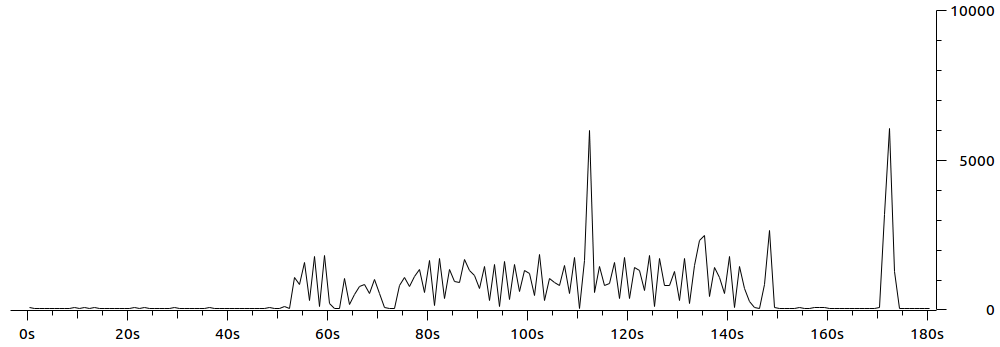
\includegraphics[keepaspectratio,width=1\textwidth]{images/file_transfer.png}
\caption{File Transfer Plot (bytes/second)}
\label{fig:file_transfer}
\end{figure}
The figure \ref{fig:file_transfer} represents a complete file transfer (the file has 7.2MB). Although the file is readable and the operation succeeds in a short amount of time (due to caching), the file transfer itself takes a bit more time. For this experiment we used 3 nodes, one connected via wireless and two planet lab nodes. We can observe that the file transfer rate is somehow smooth. However, there are two similar pinches (at 111s and 116s). We believe that they might be caused by flushing and retrieving the metadata. However, it could also be some TomP2P issue. We decided not to evaluate the transfer time with different sizes or different block sizes since we are limiting the writes and thus, the speed is determined by our parameters (now it is 160KB/s). \\
The following is the convergence time obtained for different sized networks, where each node sends a gossip message every second. The peer is randomly chosen between all the peers each node knows.\\

\begin{tabular}{|c|c|}
  \hline  
  \textbf{Number of nodes} & \textbf{Convergence time (s)} \\ \hline             
  3 & 4 \\
  4 & 6 \\
  5 & 4 \\
  6 & 5 \\
  7 & 12 \\
  8 & 15 \\
  9 & 25 \\
  \hline  
\end{tabular}\\

We also tested with a setup of 1 gossip message every 2 seconds, whose results proved only that the converge time doubles, as the rate of exchange is two times slower.
Because the number of peers is randomly chosen amongst all the peers a node knows, the convergence time seems to explode with the number of peers in the network, even though we didn't test with enough peers to reach the maximum amount of peers any node can know to find a limit to this value.\\
\begin{tabular}{l}
  \hline  
  \textbf{Gossip Query} \\ \hline             
  Num of nodes = 8.999119 \\
  Total num users = 1.163099 \\
  Total num active users = 1.000005 \\
  Avg num files per node = 0.000000 \\
  Avg num MB per node = 0.000000 \\
  \hline  
\end{tabular}\\
Here we can see a result of a gossip query to a node, after 24 seconds, on a 9 node network.
As we can see the value of the total number of users is slightly off. But the others are at
the ending stages of convergence.\\
These tests furthered our knowledge regarding the replicas. We knew the PeerMaker had 5 replication threads, which lead us to the conclusion that the replication factor was 5. During these tests, with 8 server nodes and one client node (with fuse) we found out information about the client being maintained in 6 of the nodes, consistently. So in fact, besides the information maintained by the node whose id matches the id hash of the object stored, there are 5 additional replicas in other nodes. So for every bit stored there are actually 6 bits in the network. And this value is what we need to divide when we present the gossip results.



%%%%%%%%%%%%%%%%%%%%%%%%%%%%%%%%%%%%%%%%%%%%%%%%%%%%%%%%%%%%%%%%%%%%%%%%%%%%%%%
% Section:  Conclusions
%%%%%%%%%%%%%%%%%%%%%%%%%%%%%%%%%%%%%%%%%%%%%%%%%%%%%%%%%%%%%%%%%%%%%%%%%%%%%%%
\section{Conclusions}
In a general view, we can say that we achieved a pretty good result, in a way that we accomplished all that it was asked in the project description.
More in detail, the choices made were also very efficient in solving our problems, with its strengths and weaknesses already explained. Looking to the experimental results also shows that we achieved good results, as the system responded within the expected parameters.

\end{document}
